\documentclass[letterpaper, 10 pt, conference]{ieeeconf}  % Comment this line out if you need a4paper
\IEEEoverridecommandlockouts
\overrideIEEEmargins                                      % Needed to meet printer requirements.

%\usepackage{graphics} % for pdf, bitmapped graphics files
%\usepackage{epsfig} % for postscript graphics files
%\usepackage{mathptmx} % assumes new font selection scheme installed
%\usepackage{times} % assumes new font selection scheme installed
%\usepackage{amsmath} % assumes amsmath package installed
%\usepackage{amssymb}  % assumes amsmath package installed
%\usepackage{amsthm}
%\usepackage[style=ieee]{biblatex}
%\addbibresource{references.bib}
%
%%\theoremstyle{definition}
%%\newtheorem{definition}{Definition}[section]

%\usepackage{amssymb}
%\usepackage{graphicx}
%\usepackage{epstopdf}
%\usepackage{amsmath}
%\usepackage{subfigure}
%\usepackage{multirow}
%\usepackage{pbox}
%\usepackage{algorithm}
%\usepackage{algpseudocode}
%\usepackage{bm}
%\usepackage{url}


%%%%%%

%\documentclass[conference]{IEEEtran}
%
\usepackage{graphicx}
\usepackage{epstopdf}
\usepackage{amsmath}
\usepackage{amssymb}
\usepackage{subfigure}
\usepackage{multirow}
\usepackage{pbox}
\usepackage{algorithm}
\usepackage{algorithmic}
%\usepackage{algpseudocode}
\usepackage{bm}
\usepackage{url}
\newcommand\NB[1]{$\spadesuit$\footnote{NB: #1}}
\newcommand\RP[1]{$\clubsuit$\footnote{RP: #1}}

\newcommand{\R}{\mathbb{R}}
\newcommand{\Z}{\mathbb {Z}}
\newcommand{\D}{\mathbb {D}}
\newcommand{\N}{\mathbb {N}}

\newtheorem{problem}{Problem}
\newtheorem{lemma}{Lemma}

\DeclareMathOperator*{\argmin}{arg\,min}
\DeclareMathOperator*{\argmax}{arg\,max}

\renewcommand{\baselinestretch}{0.95}


%\usepackage{graphicx}
%\usepackage{amsmath}
%\usepackage{mathrsfs}
%\usepackage{array}
%\usepackage{enumerate}
%\DeclareMathOperator*{\argmin}{arg\,min}
%\DeclareMathOperator*{\argmax}{arg\,max}
%\usepackage{amssymb}
%\usepackage{mathtools}
%\usepackage{breqn}
%\usepackage{algorithm}
%\usepackage{algorithmic}
%\usepackage{varwidth}
%\usepackage{subcaption}
%%\usepackage{subfigure}
%\newtheorem{lemma}{Lemma}
%\makeatletter
%\def\BState{\State\hskip-\ALG@thistlm}
%\makeatother
%%\bibliographystyle{ieeetr}


%\bibliographystyle{IEEEtran}


%\newcommand\NB[1]{$\spadesuit$\footnote{NB: #1}}
%\newcommand\RP[1]{$\clubsuit$\footnote{RP: #1}}
%
%\newcommand*{\Z}{\mathbb{Z}}
%\newcommand*{\N}{\mathbb{N}}
% reference package for bibtex

%\usepackage{biblatex}
%\addbibresource{mybibliography.bib}

%\usepackage[
%backend=biber,
%style=numeric,
%sorting=ynt
%]{biblatex}

%\addbibresource{mybibliography.bib}


% correct bad hyphenation here
\hyphenation{op-tical net-works semi-conduc-tor}


\begin{document}
%
% paper title
% Titles are generally capitalized except for words such as a, an, and, as,
% at, but, by, for, in, nor, of, on, or, the, to and up, which are usually
% not capitalized unless they are the first or last word of the title.
% Linebreaks \\ can be used within to get better formatting as desired.
% Do not put math or special symbols in the title.
%\title{Using Hidden Markov Models to Improve Autonomous Vehicle Decision Making - Problem Formulation}
%\title{A Hidden Markov Models-based Approach for Automotive Predictive and Assistive Control}
%\title{\LARGE \bf A Hidden Markov Model-based Approach for Predictive and Assistive Control in Semi-Autonomous Vehicles}
\title{\LARGE \bf A Hidden Markov Model-based Monitor for Predictive and Assistive Control of Hybrid Autonomous Systems}
\author{Rahul Peddi and Nicola Bezzo%
\thanks{Rahul Peddi and Nicola Bezzo are with the Department of Systems and Information Engineering and the Charles L. Brown Department of Electrical and Computer Engineering, University of Virginia, Charlottesville, VA 22904, USA. Email: {\tt \{rp3cy, nb6be\}@virginia.edu}}}



%\author{\IEEEauthorblockN{Rahul Peddi$^1$ and Nicola Bezzo$^{1,2}$} 
%\IEEEauthorblockA{
%\small
%$^1$Department of Systems and Information Engineering\\
%\small
%$^2$Department of Electrical and Computer Engineering\\
%\small
%University of Virginia\\
%Email: \{rp3cy, nbezzo\}@virginia.edu}}
%\hyphenation{u-sing}


\maketitle

% As a general rule, do not put math, special symbols or citations
% in the abstract
\begin{abstract}

Hybrid Autonomous Vehicles (HAVs) are systems in which control authority is shared between a human user and an onboard computer. In such systems, users can sometimes pass errant commands that compromise the integrity and safety of the system. In this paper, we develop a monitor for assessing and predicting the future states of other vehicles that are sharing the same task space of the HAV, and correct the user's actions to ensure safety (i.e., no collisions). We propose a framework that uses the Hidden Markov Model (HMM) theory to predict and estimate the risk and trust associated with future states. A switching strategy is also proposed to alternate between human input and autonomous input when risk is above a certain threshold. While the risk is within the safety threshold, the user is allowed to control input. The proposed approach is validated with simulations for an automotive setting with multiple vehicles that have different behaviors.



\end{abstract}
%\NB{abstract should present the problem with a little motivation and the approach with the technique and briefly mention the results}
% no keywords

% For peer review papers, you can put extra information on the cover
% page as needed:
% \ifCLASSOPTIONpeerreview
% \begin{center} \bfseries EDICS Category: 3-BBND \end{center}
% \fi
%
% For peerreview papers, this IEEEtran command inserts a page break and
% creates the second title. It will be ignored for other modes.
\IEEEpeerreviewmaketitle

\section{Introduction}
%\NB{intro needs to be rewritten...follow my comments below}
% no \IEEEPARstart

 In recent years, robotic systems have become more precise and reliable, and as a result they are used in many fields, including military, industry, and even as consumer electronics. Aerial vehicles can be used for search and rescue missions or package delivery and intelligent ground vehicles can be used for driving safety and consumer convenience applications like robotic vacuum cleaners. Many of these robotic systems are capable of autonomous behaviors, but the level of autonomy varies from system to system. For instance, modern consumer vehicles are often equipped with Adaptive Cruise Control (ACC)\cite{acc} or Advanced Driver Assistance (ADA)\cite{adas} capabilities - both of which consider a human in the loop with different levels of involvement. Humans can affect the performance, safety, and security of remote and locally-operated vehicles (cars, military drones). For aerial vehicles, nearly $33$\% of accidents implicate human error, as per the Federal Aviation Administration. \cite{aviacc}. Data from the National Highway Traffic Safety Administration in 2016 suggests that $94\%$ of crashes on the road are caused by human error \cite{nhtsa}. Of these crashes, $74\%$ are attributed to recognition and decision errors - meaning the user either did not have an understanding of the road conditions or made an unsafe decision. Thus, the human is considered as a disturbance in such systems. One solution would be to make every vehicle on the road fully autonomous, without a human in the loop. Full autonomy, however, may not
be completely possible for every application, and even if it is the ultimate goal, mixed scenarios (i.e., autonomous and manned vehicles sharing the same road), are inevitable. In this paper, we develop a monitor to assess safety in multi-vehicle operations, propose a switching approach to decide between user and autonomous behavior, deploy a safe input at all times, and avoid undesired situations (e.g., collisions).

Although our approach is general for any cyber-physical system (CPS), we focus on hybrid autonomous systems in which at any time either the user or the onboard autonomous controller has full control of the vehicle. The proposed monitor needs to predict what every other vehicle will do, determine the trust of the predictions, predict the user's actions' consequences, assess their risk, and intervene, if the risk reaches the established threshold. We deploy the proposed technique in an automotive case study in which a vehicle is on a road with other vehicles that have different behaviors similar to the case depicted in Fig.\ref{fig:hiway}.

In this figure, a user is driving a vehicle (magenta car) behind a slower vehicle (white car). In this case, both actions presented in Fig.\ref{fig:hiway} may appear safe to a driver at the moment, as indicated by the red circle; however, one of the lane changes is considerably riskier in the future because a rapidly approaching vehicle (blue car) could enter the same space as the user's vehicle (i.e., creating a collision). 

Our contribution is twofold:
    \begin{itemize}
    \item{we develop a prediction method that can effectively and efficiently estimate the future positions, the risk, and trust associated with the predictions of surrounding vehicles;} %\NB{and the risk and trust associated with these prediction}
    \item{we design a switching framework that determines the appropriate input to use and the time to switch between user and autonomous behaviors.} %\NB{change this. What you mean the severity? }
    \end{itemize}


\begin{figure}[h]
    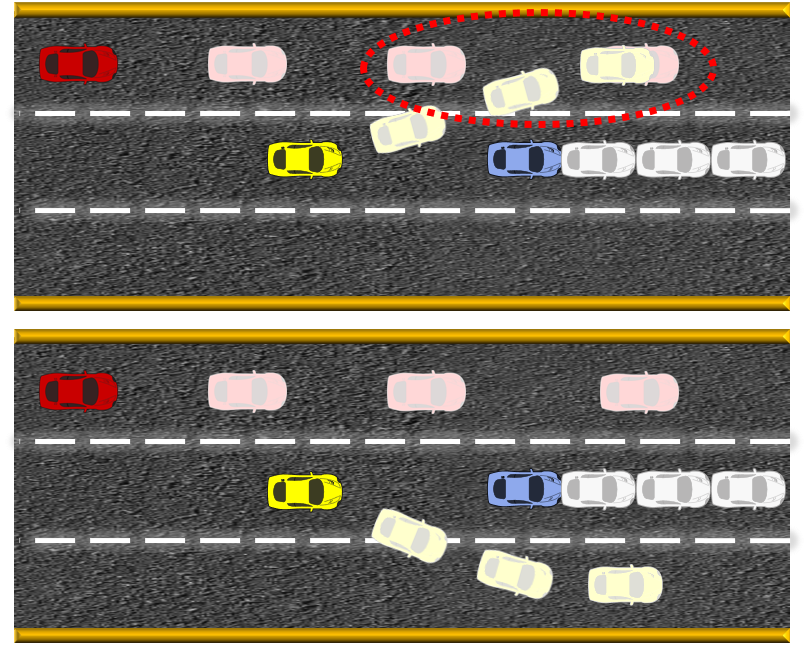
\includegraphics[width=0.48\textwidth]{fig/highway.png}
    \caption{Pictorial representation of the motivation behind this work. On the left, a vehicle may enter unsafe states due to human error. On the right, the desired outcome is displayed in which an autonomous controller takes over when the risk is above a certain threshold.}
    \label{fig:hiway}
\end{figure}

    
   The rest of this paper is organized as follows: in Section \ref{sec:relatedwork}, we discuss related work, and in Section \ref{sec:probform}, we formally define the problem. In Sections \ref{sec:approach}-\ref{sec:adapt}, we discuss each component of our approach. Our results are then demonstrated with MATLAB simulations in Section \ref{sec:sims}. Lastly, we discuss our conclusions and future work in Section \ref{sec:concs}.%\NB{fix this part}


\section{Related Work} \label{sec:relatedwork}

The study of semi-autonomous and autonomous vehicles has been growing in recent years. As these options have become more available to the average consumer, driving environments have become more mixed. Researchers approach such environments from different viewpoints: improving the knowledge about the environment (i.e., prediction) and those that involve controlling for such environments (i.e., autonomy).

The authors in \cite{mpc} use velocity predictions derived from artificial neural networks and GPS systems for Model Predictive Control (MPC), which is presented as a computationally expensive optimization problem, and the predictions can only be reliably evaluated for one vehicle at a time. The authors in \cite{velnn} and \cite{veldatadriv} take a data science approach and use large data-sets along with very specific traffic information in order to make predictions. The use of a Hidden Markov Model (HMM)-based approach for prediction is done in \cite{lanhmm}, where the authors develop an approach that treats a vehicle as a hybrid state system in order to predict the trajectory of a certain behavior. This is done assuming knowledge of multiple states that cannot be observed from outside of the system. In \cite{woohmm}, motivated by previous work in HMMs, the authors discuss using a simplified form of the hybrid state system with an HMM to improve lane change prediction for a single vehicle. In our work, we consider the problem of predicting future velocity and when lane changes are expected by leveraging similar theories presented in \cite{mpc} and \cite{woohmm}.

In terms of controlling vehicles in such environments, the authors in \cite{qmdp} use a Point-Based Markov Decision Process (QMDP) to estimate dangerous situations and react with the appropriate autonomous driving behavior in single-lane situations. The QMDP process employs a robust but computationally expensive value iteration algorithm in order to select the safest action in a single lane situation. In \cite{predcost}, the authors present a prediction and cost-based (PCB) control strategy for autonomous vehicles given a known set of predicted scenarios. In this vein, \cite{vfh*} discusses reliable obstacle avoidance methods given that obstacle locations and characteristics which are known based on artificial physics methods. In \cite{takeover}, with a human-factors based approach, the authors show multiple ways that take-over requests can be generated in partially autonomous vehicles, including performance based and environment based characteristics. In our work, we leverage the idea of sharing control from \cite{takeover}, along with the theories in \cite{vfh*} to control for future unsafe scenarios.

    
\section{Problem Formulation} \label{sec:probform}
 
In this work we are interested in finding an approach to proactively guarantee safety (i.e., a collision does not occur) in multi-vehicle systems operations. We focus on manned vehicles employing a hybrid autonomy scheme as defined in \cite{corke} in which the control authority is shared between the human and the onboard computer. For the sake of brevity, we denote this class of vehicles as {\em hybrid autonomous vehicles} (HAVs). In our scheme, the onboard computer is used as a supervisory monitor to predict and assess safety, and correct undesired human behaviors that may lead to unsafe situations that compromise the system's integrity. 

Formally the problem that we investigate in this work can be stated as: 

\textbf{Problem 1: \textit{Proactive Safe Assisted Planning and Control}:} 
      An HAV $h$ is moving in an environment in the presence of other vehicles $q \in R_h(t)$, where $R_h(t)$ is a time varying set of vehicles in sensing/communication range with $h$. The goal is to find a policy to:
    \begin{enumerate}
        \item  predict online other vehicles future states $s$ and their likelihood $p$. Formally, $\forall q \in R_h(t)$:
    \begin{equation}
   S_q=\{{s_q(t), s_q(t+1),..., s_q(t+T)}\}
       \end{equation}
       \begin{equation}
   P_q=\{{p_q(t), p_q(t+1),..., p_q(t+T)}\}
    \end{equation}
     where $S_q$ is the set of all states, $s_q$, and $P$ is the set of all probabilities, $p_q$ over a finite time horizon $T\in\N$.  
    \item assess the risk $0\leq r \leq1$ of a collision during $T$ and
    \item assist and intervene to correct the HAV actions to guarantee safety, i.e., obtain an input policy $U_h=\{{u_h(t), u_h(t+1),..., u_h(t+T)}\}$ such that the risk $r$ is always minimized. 
    \end{enumerate}
   In our specific multi-vehicle case, risk is a function of distance between vehicles. Hence, minimizing risk is equivalent to guaranteeing the following:

    \begin{equation}
        ||{x_h(t)-x_q(t)}|| \geq d_{\textrm{min}}
    \end{equation}
     where $x_h(t)$ and $x_q(t)$ are the positions of the HAV and the $q^{\textrm{th}}$ surrounding vehicle at time $t$, and $d_{min}$ is a minimum safe distance.    
    
    It is important to note that the vehicle that we are assisting is primarily human operated, in which the monitor should intervene only when necessary.
    Unless the HAV has a reachable state that is unsafe, which we define as a situation where $r_h(t)>r_{\max}$, where $r_{\max}$ is a user-defined threshold, we let the user perform his/her desired actions.


\section{Approach} \label{sec:approach}

Our approach is summarized in the architecture presented in Fig.~\ref{fig:app}. 
\begin{figure}[ht!]
    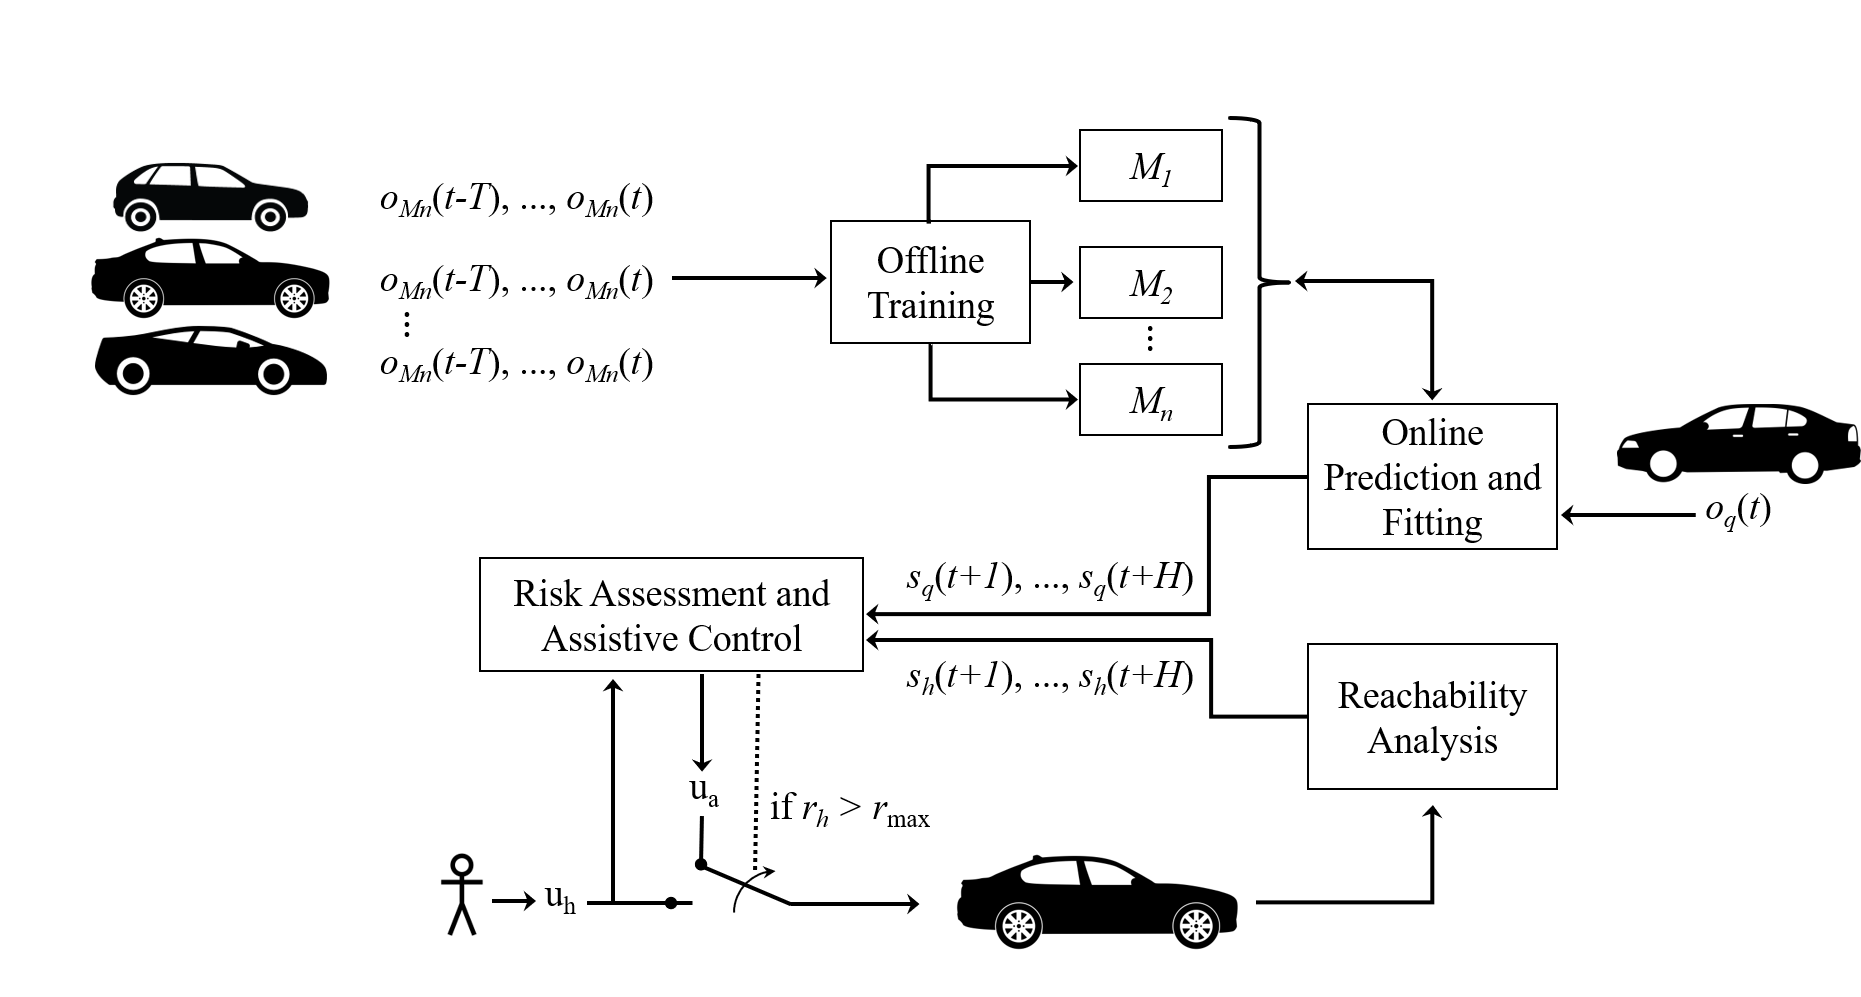
\includegraphics[width=0.48\textwidth]{fig/approach.png}
    \caption{Block Diagram of the Approach}
    \label{fig:app}
\end{figure}

We leverage a history of offline observations, $\{o(t-T),\ldots,o(t)\}$, to build different models, $\{M_1,\ldots,M_n\}$, that are then used online to recognize and predict new vehicles' behaviors. Based on these predictions, and the user's input $u_h$, a monitor predicts and assesses whether $h$ could enter any unsafe state. If such an unsafe action is detected, an autonomous control action, $u_a$, is deployed to assist and correct the user's intention. In the next sections, we will go over this framework, explaining in detail each block presented in Fig.~\ref{fig:app}.

\section{HMM-based Training Framework} \label{sec:fmwk}
 In order to predict future states of other vehicles, we perform offline training of data collected over a horizon $T$ to extract and differentiate between multiple behavioral models. To this end, we propose a modified version of the Hidden Markov Model (HMM) \cite{woohmm} which can be described by a tuple $\langle \mathcal{O},\mathcal{S},\mathcal{C},\mathcal{G},\mathcal{P},\mathcal{B} \rangle$  where:
\begin{itemize}
    \item $\mathcal{O}\in\mathbb{R}^T$ is a finite set of observed states $o(t)$ collected over a finite past time horizon $T$, $\mathcal{O} = \{ o(t-T), o(t-T+1), \ldots, o(t)\}$. 
    \item  $\mathcal{S}\in\mathbb{R}^n$ is a finite set of $n$ unique values that $\mathcal{O}$ can obtain, i.e., $\{s_i,s_j\} \in \mathcal{S} \vert s_i \neq s_j$ with $i\neq j$,and $i,j = 1,\ldots,n$, with $n \in \mathbb{N}$.
    \item $\mathcal{C}\in\mathbb{R}^T$
    is the finite set of emissions, or inferences $c(t)$ that relate to the action taken each state, and $\mathcal{C} = \{ c(t-T), c(t-T+1), \ldots, c(t)\}$.
    \item $\mathcal{G}\in\mathbb{R}^m$ is a finite set of $m$ unique inferences that $\mathcal{C}$ can obtain. and $g_k \in \mathcal{S}$, where $k = 1,\ldots,m$, with $m \in \mathbb{N}$. 
    \item $\mathcal{P}\in\mathbb{R}^{n\times n}$ is a transition probability matrix. This matrix describes the probability of entering a certain state, $s_{j}$, while currently in a particular state $s_{i}$, denoted as $s_j \to s_i$, defined by:
        \begin{equation}
            p_{ij} = P(s_j\to s_i)
        \end{equation}
        These probabilities are initialized as $1/n$. Each transition probability is calculated by counting the occurrences of each state transition over all transitions from that state:
        \begin{equation} \label{eq:transbuild}
            p_{ij} = N_{ij}/N^*_{i}
        \end{equation}
        where $N_{ij}$ represents the total number of transitions, $s_j \to s_i$, over $T$ and $N^*_{i}$ is the total number of transitions from $s_i$ to any state, and $N_{ij} \leq N^*_{i} \leq T$. The state transition matrix is right-stochastic, meaning the sum of all rows is $1$ and is of the form:
        \begin{equation}
            \mathcal{P} = 
                    \begin{bmatrix}
                        p_{11} & \dots & p_{1n} \\
                        \vdots &\ddots & \\
                        p_{n1} &    & p_{nn}
                    \end{bmatrix}
        \end{equation}
    \item $\mathcal{B}\in\mathbb{R}^{n\times m}$ is the emission matrix, which lists the probability $b_{ik}$ of obtaining emission $g_k$ given state $s_i$:
        \begin{equation} \label{eq:obsref}
            b_{ik} = P(g_k(t+1) \vert s_i(t))
        \end{equation}
        where $i = 1,\ldots,n$. These probabilities are initialized as $1/m$, and are calculated in a similar way to (\ref{eq:transbuild}):
        \begin{equation} \label{eq:obsbuild}
            b_{ik} = N_{g_{ik}}/N^*_{g_{i}}
        \end{equation} 
        where $N_{g_{ik}} \leq N^*_{g_{i}} \leq T$.
        \begin{equation}
            \mathcal{B} = 
                    \begin{bmatrix}
                        b_{11} & \dots & b_{1m} \\
                        \vdots & \ddots & \\
                        b_{n1} &    & b_{nm}
                    \end{bmatrix}
        \end{equation}
\end{itemize}

This framework is executed over $T$ and a set of parameters is obtained: $\langle \mathcal{P}, \mathcal{B} \rangle$. Our framework is different from a traditional HMM because the states are not hidden, and we know exactly the relationship between states and their corresponding inferences. Because we have all the states and transitions a priori, we can learn the parameters of multiple models offline. The general pictorial representation of the framework is shown in Fig.~\ref{fig:hmm}. In this image, nodes labeled $s$ represent the states ($\mathcal{S}$), while those labeled $g$ represent the emissions ($\mathcal{G}$). The lines with the label $p$ are the transition probabilities between states, and those labeled $b$ are the probabilities that each of the connected observations are associated with connected states.
\begin{figure}[h]
    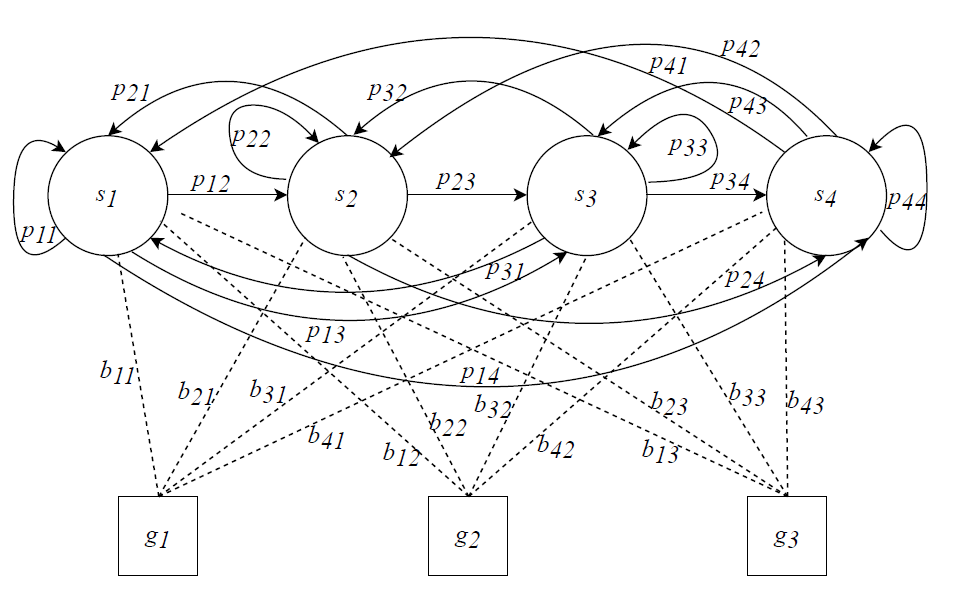
\includegraphics[width=0.48\textwidth]{fig/ahmm.png}
    \caption{General Representation of the Hidden Markov Model (HMM) for our framework}
    \label{fig:hmm}
\end{figure}

The specific environment that we are studying involves multiple vehicles that can change their velocities and their lanes.

Our goal is to predict future velocities $v$ and lanes $l$ of all the surrounding vehicles $q\in R_h$. In this case, $S_v = \{v_1,\ldots, v_n\}$, $S_d = \{d_1,\ldots,d_n\}$, $S_l = \{l_1,\ldots,l_n\}$, where $S_v$ is the set of velocities, $S_d$ is the set of distances between vehicles, and $S_l$ is the set of lanes. The emissions reflect the actions performed between two consecutive states. In our case, emissions are associated to the following vehicle input behaviors: changes in velocity and changes in lane.
For velocity we consider the following 3 emissions,

\begin{itemize}
    \item[$b_1^v$] {Increasing Velocity if $v(t) > v(t-1)+\delta_v$} 
    \item[$b_2^v$] {Decreasing Velocity if $v(t) < v(t-1)-\delta_v$}
    \item[$b_3^v$] {Maintaining Velocity if $v(t-1)-\delta_v \leq v(t) \leq v(t-1)+\delta_v$}
\end{itemize}
%\NB{formalize...$v(t-1)+\delta_v$ etc}
%\NB{give a name to this emissions...i.e. $b_{1}^v, b_{2}^v$}
%\NB{if not where}
where $\delta_v\in\mathbb{R}^+$ and reflects the change in velocity from one step to another.

For the lanes, the following 3 emissions are considered:

\begin{enumerate}
    \item[$b_1^l$] Changing Left if $l(t) < l(t-1)$
    \item[$b_2^l$] Changing Right if $l(t) > l(t-1)$
    \item[$b_3^l$] Not Changing if  $l(t) = l(t-1)$
\end{enumerate}
where we assume that lanes are modeled in increasing order from left to right; i.e. the leftmost lane is $1$ and the rightmost lane is $n$.


\section{HMM-Based Online Prediction and Model Updates} \label{sec:ahmmpredupdate}
  Using the framework outlined in Section \ref{sec:fmwk}, given enough observations, we can extract a model for each surrounding vehicle. This model can be used online to predict future states of the system, and this is achieved by collecting more observations online. These online observed states can then be applied to the pre-trained emission and transition matrices as lookup tables to obtain the most likely future state. Each future state is determined as:
 
\begin{equation} \label{eq:pred}
    s(t+1) = s_j \in S \vert p_{ij}=\max_p(\mathcal{P}_i*)
\end{equation}

The likelihood that $s(t+1)$ is indeed the future state is denoted as:
\begin{equation}
    P[ s(t+1) = s_j]=\max_p(\mathcal{P}_i*)
\end{equation}

In the event that \eqref{eq:pred} returns more than one value, we cross-reference the states with the emission matrix, $\mathcal{B}$ as follows: 
\begin{equation} \label{eq:pred2}
    s(t+1)=s_j\vert g_{ij} = \max_b(\mathcal{B}_i*)    
\end{equation}


In the event that \eqref{eq:pred2} still returns more than one state, we choose the more dangerous transition, which depends on the specific application. For instance, in our case, the more dangerous transition is one that reduces distance between the user's vehicle and other vehicles.

Using this approach, we can predict a series of future states over any horizon $H$ by assuming that each prediction for $t+1$ is correct. We re-use the emission and transition matrices to predict a sequence of future states up to horizon $H$.
It is, however, important to note that as $H$ is increased, every successive prediction tends to be less accurate, as the sequence of future predictions is built assuming each of the previous predictions is correct.

Algorithm~\ref{alg:pred} shows how we carry forward this prediction through $H$. In this algorithm, an observed state, $s(t) = s_i$, is used in %\NB{in not with} 
$\mathcal P$ and $\mathcal B$ to find the most likely next state, $s(t+1) = s*_{j}$ %\NB{$s_j^*$}.
At the following step, $s(t+2)$ is calculated using the previously predicted $s_{j^*}$. This process is repeated up to $t+H$, obtaining a series $\{s(t+1),\ldots,s(t+H)\}$ of future states.
%\NB{I think we can remove this if you have explained the procedure well before}
%\NB{assuming that next observation is be the predicted $s(t+1)$}. This process is repeated up to $t+H$.

\begin{algorithm}[ht!]
\caption{Future State Prediction} \label{alg:pred}
\begin{algorithmic}[1]
\WHILE{$t\leq t+H$}
\STATE $s(t) = s_i$
\STATE $s(t+1) = s_j \in S \vert p_{ij}=\max(\mathcal{P}_i)$
\IF{$s_j$ is not a singleton, $s_j\in S$}
\STATE $s(t+1)=s_j\in S\vert p_{ij}=\max(\mathcal{P}_i) \land g_{ij} = \max(\mathcal{B}_i)$
\STATE $s(t+1) \gets s_{j}$
\IF{$s_j$ is not a singleton}
\STATE $s(t+1) = \max_{s_j}S,\forall s_j\in S\vert p_{ij}=\max(\mathcal{P}_i)$
\ENDIF
\ENDIF
\STATE $s_i = s(t+1)$
\STATE $t \gets t+1$
\ENDWHILE
\end{algorithmic}
\end{algorithm}


It is, however, possible that the online predictions are incorrect, indicating that the offline model does not accurately represent the system we are currently observing. In order to alleviate this issue, $\mathcal{P}$ and $\mathcal{B}$ are updated online. This is achieved by using \eqref{eq:transbuild} and \eqref{eq:obsbuild}, where we adjust $N_{ij}$ and $N_{ik}$, thus also changing $p_{ij}$ and $b_{ij}$. As a result, new transition and emission matrices $\mathcal{P'}$ and $\mathcal{B'}$ are created at each iteration to reflect the updates. In addition, we use a sliding window approach such that the size of the training set is always a constant $T$. %\NB{is always constant $T$}\NB{remove this last part}.
The training set is kept the same size in order to retain computational efficiency and to avoid accumulating older and less reliable data. Another option would be to discount older data, however we decide not to use this method in this paper because the transition and emission matrices will grow larger, decreasing the efficiency of the proposed method. 

\section{Online Model Fitting}\label{sec:omf}
Using the framework described in Sections \ref{sec:fmwk} and \ref{sec:ahmmpredupdate}, we can extract a model that captures the behavior of a system that we have been observing for $T$. Multiple models $\mathcal{M} = \{M_1,\ldots,M_m\}$ can be extracted using several data sets. Each of these models are characterized by unique transition and emission matrices to capture $m$ different behaviors which will be used at run-time to predict the behavior of any new observed system.

The transition and emission matrices of these models are denoted as follows:
\begin{equation}
    \hat{\mathcal{P}} = \{\mathcal{P}_1,\ldots,\mathcal{P}_m\}
\end{equation}
\begin{equation}
    \hat{\mathcal{B}} = \{\mathcal{B}_1,\ldots,\mathcal{B}_{m}\}
\end{equation}

%\NB{where $M\in\mathbb{N}$ represents the number of models}.

During run-time, we observe new measurements of other vehicles. The challenge here becomes fitting each vehicle's observations to one of the offline models. Until we have enough observations, the prediction may not be accurate. Thus, we need to take into account possible errors in the prediction, $e_i$ as we are matching the vehicle behavior with the offline models. 

We treat any vehicle observed online as a new system from which we are interested to compute a model, hence we follow the same procedure in Section \ref{sec:fmwk} to extract transition and emission matrices. Each element of transition matrix, $\tilde{\mathcal{P}}(t)\in\mathbb{R}^{n\times n}$, is initialized to $\tilde{p}_{ij} = 1/n$, where $i,j = 1,\ldots,n$. Similarly, each element of the emission matrix,  $\tilde{\mathcal{B}}(t)\in\mathbb{R}^{n\times m}$, is initialized to $\tilde{b}_{ik}= 1/m$, where $i = 1,\ldots,n$ and $k=1,\ldots,m$. At each iteration, these matrices are updated using the method discussed in \ref{sec:ahmmpredupdate}, and are then compared with those of the pre-trained models, $\hat{\mathcal{P}}$ and $\hat{\mathcal{B}}$.

The most similar model is chosen to predict the behavior of the observed system. To obtain this model, the following error is computed at every iteration:
 %\NB{how are these matrices initialized? We need to show the initial expression of these matrices 1/n ...}
\begin{equation} \label{eq:pnorm}
    \forall{P_i} \in \hat{\mathcal{P}}: e_i = \frac{1}{n}\lVert\tilde{\mathcal{P}}(t)-\mathcal{P}_{i}\rVert_{2}
\end{equation}

where $\frac{1}{n}$ is the inverse of the number of columns in $\mathcal{P}$ and is used to normalize the error, $\lVert \cdot \rVert_2$ is the $l_2$ matrix norm, which in our case, represents the distance (i.e. error) between transition matrices of the observed model and the offline models. This error indicates the confidence we have in each model. A higher error indicates more uncertainty that our predictions will be correct.

Combining all errors, we obtain $\hat{e} = \{e_1,\ldots,e_m\}$. To make predictions, we select the model $M^*$ with the lowest error:

\begin{equation}
    M^*=M_i\in\mathcal{M}\vert e_i = \min_e(\hat{e})
\end{equation}

  Given this model, the associated transition and emission matrices, $\mathcal{P}_{i}$ and $\mathcal{B}_{i}$ are used in order to make predictions. The procedure to predict future states is shown in Algorithm~\ref{alg:pred}. In addition, a trust measure for the selected model is determined as:
  \begin{equation}
    \rho = 1-e_i
 \end{equation}
 where $e_i$ is the error associated with $M^* = M_i$. Because trust is the complement of error, the model with the lowest error, $M^*$ also has the highest trust. This trust measure is utilized in Section \ref{sec:adapt} to determine risk.

\begin{lemma}
Given the optimal model $M^*$, we guarantee that we can trust with a factor of $/rho$ that the predictions made using Algorithm~\ref{alg:pred} will be accurate with probability $\mathbf{P}$.
\end{lemma}

\begin{proof}
Using Algorithm~\ref{alg:pred} on the transition and emission matrices of model $M^*$, we obtain predicted future states up to time horizon $T$, $\{s(t+1),s(t+2),\ldots,(t+T)\}$
\end{proof}

%Using \eqref{eq:riskdistribution}, we generate a risk distribution $\hat{\mathcal{R}}$. 
%The optimal input pair $u^*(t)=(l^*(t),v^*(t))$ is determined from $r^*(t)$ in \eqref{eq:optpt}.
%, which is the minimum of $\hat{\mathcal{R}}(1,j)$. 
%Assuming that we are in steady state, meaning trust $\rho$ is not changing, from \eqref{eq:riskcalc} we obtain:
%\vspace{-10pt}
%\begin{equation}
%\gamma_q^*(t) = \frac{1}{r^*(t)}=(\xi+1) d_q(t) \rho
%\end{equation}
%\vspace{-10pt}
%Minimizing risk means that the quantity $(\xi+1)d_q(t)$ is maximized, hence meaning that the separation between vehicles is maximized.

%Thus, the input $(l^*,v^*)$ guarantees that at each iteration the separation between $h$ and any other vehicle is maximized. Any other possible input $u(t) \neq u^*(t)$ is associated with a risk $r(t)>r^*(t)$, as defined in \eqref{eq:riskcalc}. $\forall u(t) \neq u^*(t)$, $(\xi+1)d_q(t)\leq\gamma_q^*(t)$ hence proving that $u^*(t)$ will achieve the maximum possible separation at every step.

%\end{proof}


\section{Assistive Control} \label{sec:adapt}

\subsection{Reachability Analysis}

In this work, we are interested in assessing risk of collision. In order to assess this risk we need to predict:
\begin{enumerate}
\item future states of the surrounding vehicles which are obtained by following the procedure outlined in Section \ref{sec:ahmmpredupdate} and
\item the reachable states of $h$ over a future horizon $H$.
\end{enumerate}
In some of our current work, we are using Hamilton-Jacobi reachability analysis to predict future states of a system under uncertainties \cite{esen}. In this paper, we consider a simplified approach for reachability in which we assume that:
\begin{enumerate}
\item The vehicle can move to the adjacent lane in one time step $\delta t$ \label{ass:i}
\item future variations of velocity are bounded $v_h-\delta_v \leq v_h\leq v_h+\delta_v$, with $\delta_v>0$ \label{ass:ii}
\end{enumerate}
Both \ref{ass:i}. and \ref{ass:ii}. are worst case scenarios. %Assumption \ref{ass:ii} reflects a physical limitation of vehicles.
Using these assumptions, three reachable velocities can be considered as follows:
\begin{enumerate} %\NB{t+1 not i}
    \item $v_h^=(t+1)=v_h(t)$
    \item $v_h^-(t+1)=v_h(t)-\delta_v$
    \item $v_h^+(t+1)=v_h(t)+\delta_v$
\end{enumerate} 
and $\hat{V} = \{v^-(t),v_h^=(t),v^+(t)\}$, which is a time-varying set that depends on the current velocity, $v_h(t)$. Future reachable forward positions can be easily computed as $x_h(t+i)=v(t+i)\delta t$, where $\delta t$ is the sampling time, for each of the three aforementioned velocities. Reachable lanes are modeled as $\hat{L} = \{l_1,\ldots,l_n\}$, in which $n$ lanes are considered. 

\begin{figure}[ht!]
    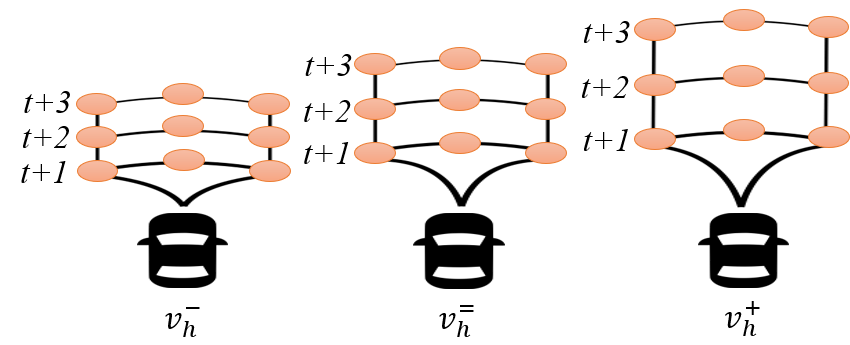
\includegraphics[width=0.48\textwidth]{fig/reach.png}
    \caption{Reachable set for each velocity}
    \label{fig:reach}
\end{figure}

Three reachable sets containing all the possible states that can be reached by $h$ are obtained. For example, if $h$ is on a 3 lane road and the prediction horizon is 3 time steps, then a total of 27 predictions are obtained, as indicated by the points in Fig. \ref{fig:reach}.

\subsection{Risk Assessment}

Risk is determined by computing the relative distance between $h$ and all vehicles $q\in R_h$ over the predictive horizon $H$. By using the approach presented in Section \ref{sec:ahmmpredupdate}, we can predict future states for all $q$ to obtain:
%\RP{Change to bar or tilde or hat for predictions}
\begin{equation}
    V_q = \{v_q(t+1),\ldots,v_q(t+H)\}
\end{equation}
\begin{equation}
    L_q = \{l_q(t+1),\ldots,l_q(t+h)\}
\end{equation}

where $V_q$ and $L_q$ are the predicted future velocities and lanes for each vehicle $q$, respectively.
Using these future velocities, we can calculate the positions of each $q$ over the horizon $H$ as $x_q(t) = v_q(t)\delta t + x_q(0)$ and obtain the predicted future positions:
\begin{equation}
    \hat{x}_q = \{x_q(t+1),\ldots,x_q(t+H)\}
\end{equation}
We can then calculate relative distance as
\begin{equation}
    \forall q \in R_h: d_q(t) = \lVert x_h(t)-x_q(t)\rVert_2
\end{equation}
where $\rVert \cdot \lVert_2$ indicates the $l_2$ vector norm. Risk is inversely proportional to distance $d_q(t)$, lane separation $l_q(t)$, and trust $\rho$. Specifically, the risk $r_q^l(t)$ associated with vehicle $q$ and lane $l$ at time $t$ is computed as follows: %\NB{what about the lanes?}

\begin{equation} \label{eq:riskcalc}
    r_{q}^{l}(t) =
    \begin{cases}
    \frac{1}{(\xi+1) d_{q}(t)\rho},  & \text{if } d_{q}(t) > 1  \\
        1,                     & \text{otherwise}  
    \end{cases}
\end{equation}

where $\xi$ is the difference in lanes between $h$ and each vehicle $q\in R_h$.
% \NB{what is this function?} 
 The values obtained from \eqref{eq:riskcalc} are calculated for each reachable velocity and position of $h$. For each $q$ and $v$, we can compute the following risk matrix: %\NB{the vehicle are arranged as follows?}:
\begin{equation} \label{eq:riskmat}
\mathcal{R}_{q}^{v}=
\begin{bmatrix}
r_q^{l_1}(t+1)  \dots  r_q^{l_n}(t+1) \\
\vdots  \ddots  \\
r_q^{l_1}(t+H)  \dots   r_q^{l_n}(t+H)
\end{bmatrix} q = 1,\ldots,m,v\in\hat{V}
\end{equation}
Combining together all of the risk matrices, we obtain the following superset $\mathcal{R}$:

\begin{equation} \label{eq:superrisk}
\mathcal{R} =
\begin{bmatrix}
\mathcal{R}_{1}^{v_h^-} & \ldots & \mathcal{R}_{m}^{v_h^-} \\
\mathcal{R}_{1}^{v_h^=} & \ldots & \mathcal{R}_{m}^{v_h^=} \\
\mathcal{R}_{1}^{v_h^+} & \ldots   & \mathcal{R}_{m}^{v_h^+}
\end{bmatrix}
\end{equation}
The representation in \eqref{eq:superrisk} suggests that multiple vehicles affect risk in our analysis. We are most concerned with the highest risk at each reachable point, which can be due to any vehicle, and is evaluated as follows: %\NB{any reachable point shown in Fig.}.
\begin{equation} \label{eq:riskdistribution}
 \hat{\mathcal{R}}(i,j) = \max\begin{pmatrix}
 \begin{bmatrix}
\mathcal{R}_{1}^{v^-}(i,j) & \ldots & \mathcal{R}_{m}^{v^-}(i,j) \\
\mathcal{R}_{1}^{v_h}(i,j) & \ldots & \mathcal{R}_{m}^{v_h}(i,j) \\
\mathcal{R}_{1}^{v^+}(i,j) & \ldots   & \mathcal{R}_{m}^{v^+}(i,j)
\end{bmatrix}\end{pmatrix}
\end{equation}

 where $i = 1,\ldots,H$, $j = 1,\ldots,n$, and $\hat{\mathcal{R}} \in \mathbb{R}^{H\times n}$.
 

 In Fig.~\ref{fig:distr}, we show an example of a risk distribution (i.e. $\hat{\mathcal{R}}$), over $H=3$ for velocity $v_h$. A risk distribution takes into account the future states of each vehicles in the time-varying set of vehicles $R_h(t)$. The road scenario (Fig.~\ref{fig:roads}) shows the user's vehicle as well as reachable points for the vehicle, as indicated by the lines labeled with timesteps. In addition, other vehicles and future predictions of those vehicles for horizon $H=3$ are also shown in the road scenario.

\begin{figure}[ht!]
	\centering
	\subfigure[Risk Distribution \label{fig:distr}]{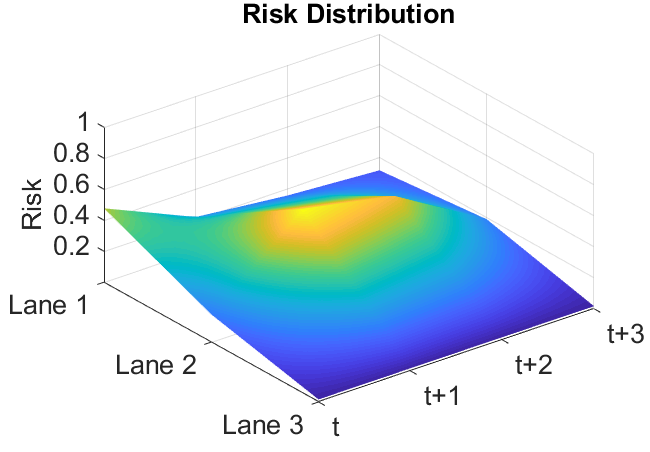
\includegraphics[width=0.45\linewidth]{fig/assist_rd.png}}
	\subfigure[Road Scenario \label{fig:roads}]{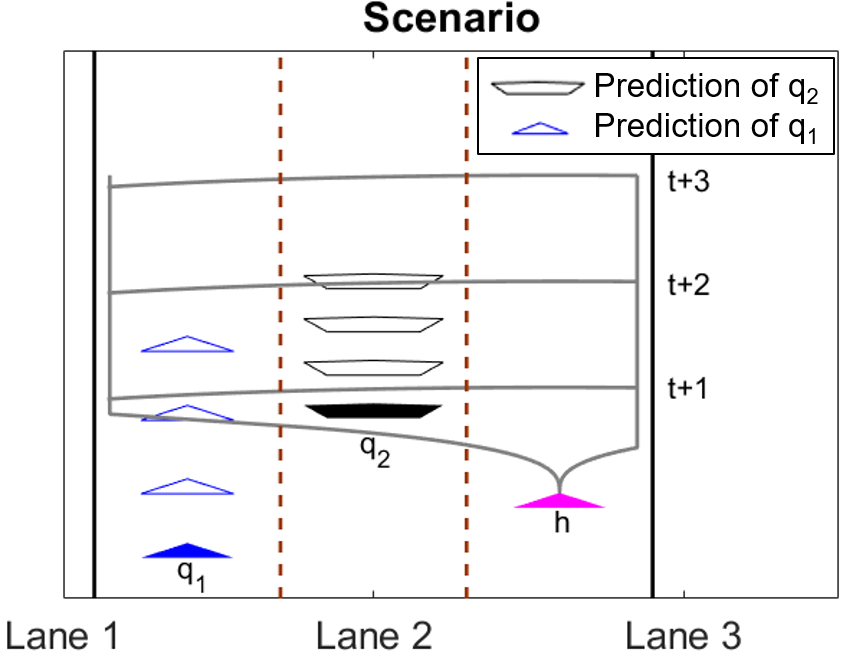
\includegraphics[width=0.4\linewidth]{fig/riskdist_rs.png}}
	\vspace{-5pt}
	\caption{Risk distribution and associated road scenario}
	\label{fig:riskd}
	\vspace{-15pt}
\end{figure}


\subsection{Adaptive User Assistance}

Given the risk distribution, we can assist our user's potentially unsafe actions to guarantee safety, by performing actions that minimize risk. In order to adapt, we need to first identify whether these actions are going to result in a dangerous situation i.e., a collision. User actions, in this case, are limited to selecting a reachable lane and velocity,
\begin{equation}
u_h(t) = (l_h(t),v_h(t)), \text{ where } l(t)\in\hat{L}, v_h(t)\in\hat{V}
\end{equation}
A user-set threshold, $r_{\max}$ is defined. If risk is below $r_{\max}$, we let the user continue his/her desired actions, and if it is above $r_{\max}$, the autonomous component in the HAV takes control of the system. Given $r_{\max}$ and the values in the risk distribution, as indicated in Figs.~\ref{fig:reach} and \ref{fig:riskd}, the input $u*(t)$ is either the user input $u_h(t)$ or the autonomous input $u_a(t)$ as follows:

\begin{equation} \label{eq:inputctrl}
    u^*(t) = \begin{cases}
    u_h(t) & \text{ if } \hat{\mathcal{R}}(i,j) < r_{\max}, \forall\hat{\mathcal{R}}(i,j)\in\hat{\mathcal{R}} \\
    u_a(t) & \text{ if } \exists~\hat{\mathcal{R}}(i,j) >= r_{\max}
    \end{cases}
\end{equation}
 
During run-time, we are monitoring $\hat{\mathcal{R}}$ to find the appropriate pair of actions (velocity and lane) that minimize risk at time $t+1$. In order to identify the safest actions, we use gradient descent on the risk distribution:
\begin{equation} \label{eq:optpt}
  r^*(t+1) = \min\{\hat{\mathcal{R}}(1,1),\ldots,\hat{\mathcal{R}}(1,n)\}  
\end{equation}
In other words, we are only concerned with the first row of $\hat{\mathcal{R}}$, which corresponds to $t+1$.
The value $r^*(t+1)$ gives information about the safest lane to enter and the safest velocity to reach. The optimal input pair can be obtained as follows, $\hat{\mathcal{R}}$:
\begin{align} \label{eq:optpair}
    l^*(t) &=  l_j\in\hat{L}\vert r^*(t) = \hat{\mathcal{R}}(1,j)\in\hat{\mathcal{R}} \nonumber \\
    v^*(t) &=  v\in\hat{V}\vert r^*(t) = \hat{\mathcal{R}}(1,j)\in\hat{\mathcal{R}}
\end{align}


At every iteration, the optimal pair $(l^*(t),v^*(t))$ is calculated. In this work, we place an emphasis on the user's risk threshold $r_{\max}$, so the autonomous input $u_a(t) = (l^*(t),v^*(t))$ is only implemented when the condition described in \eqref{eq:inputctrl} is met. By minimizing the risk at $t+1$, we ensure that the immediate action of our vehicle $h$ is always the safest option.

%\begin{lemma}
%Given a configuration where there exists a safe sequence of actions, and if any risk in this configuration is above the threshold, $ \exists~\hat{\mathcal{R}}(i,j) >= r_{\max}$ over horizon $H$, the approach in Section \ref{sec:adapt} guarantees that the system is always going to be safe. This is a probabilistic guarantee that hinges on the trust measure $\rho$ of our predictions.

%\end{lemma}

%\begin{proof}
%Using \eqref{eq:riskdistribution}, we generate a risk distribution $\hat{\mathcal{R}}$. 
%The optimal input pair $u^*(t)=(l^*(t),v^*(t))$ is determined from $r^*(t)$ in \eqref{eq:optpt}.
%, which is the minimum of $\hat{\mathcal{R}}(1,j)$. 
%Assuming that we are in steady state, meaning trust $\rho$ is not changing, from \eqref{eq:riskcalc} we obtain:
%\vspace{-10pt}
%\begin{equation}
%\gamma_q^*(t) = \frac{1}{r^*(t)}=(\xi+1) d_q(t) \rho
%\end{equation}
%\vspace{-10pt}
%Minimizing risk means that the quantity $(\xi+1)d_q(t)$ is maximized, hence meaning that the separation between vehicles is maximized.

%Thus, the input $(l^*,v^*)$ guarantees that at each iteration the separation between $h$ and any other vehicle is maximized. Any other possible input $u(t) \neq u^*(t)$ is associated with a risk $r(t)>r^*(t)$, as defined in \eqref{eq:riskcalc}. $\forall u(t) \neq u^*(t)$, $(\xi+1)d_q(t)\leq\gamma_q^*(t)$ hence proving that $u^*(t)$ will achieve the maximum possible separation at every step.

%\end{proof}

\section{Simulations} \label{sec:sims}
%\vspace{-30pt}
In the following simulations we validate the proposed monitoring and adaptive approach presented in Section \ref{sec:approach} on an automotive case study. First, we discuss how different vehicle's models are trained and validated (from Sections \ref{sec:fmwk} and \ref{sec:ahmmpredupdate}). Then, we show an example of online model fitting (from Section \ref{sec:omf}) given a known pre-trained set of models. Finally, we demonstrate the risk estimate and assistive behaviors (from Section \ref{sec:adapt}) for a safety critical automotive case study on a road with multiple vehicles and demonstrate the validity of our framework.

\vspace{-5pt}
\subsection{Model Training Example}
In order to train different vehicle models, we used an environment featuring $6$ stationary obstacles. A test vehicle with a predefined behavior was driven through the environment, while avoiding these obstacles. The vehicle's velocity, lane changes, and distance to each obstacle was observed for a training period of $T=700$ iterations. During this period, the framework discussed in Section \ref{sec:fmwk} was executed and $\mathcal P$ and $\mathcal B$ matrices were generated for both velocity measurements and lane change measurements. The effectiveness of the generated transition and emission matrices was validated online against the same vehicle running over a new environment with $9$ obstacles. Following the scheme in Section \ref{sec:ahmmpredupdate} a one step prediction was computed and compared with the vehicle's ground truth velocity and position.
Fig.~\ref{fig:trainvel} shows the absolute error between actual and estimated velocities while Fig.~\ref{fig:trainpos} shows the absolute error between the predicted and actual position of the vehicle. The resulting root mean square error (RMSE) for forward position estimates was recorded to $0.3927$m.

\begin{figure}[ht!]
	\centering
	\subfigure[The error between the velocity of the actual model and estimated velocities \label{fig:trainvel}]{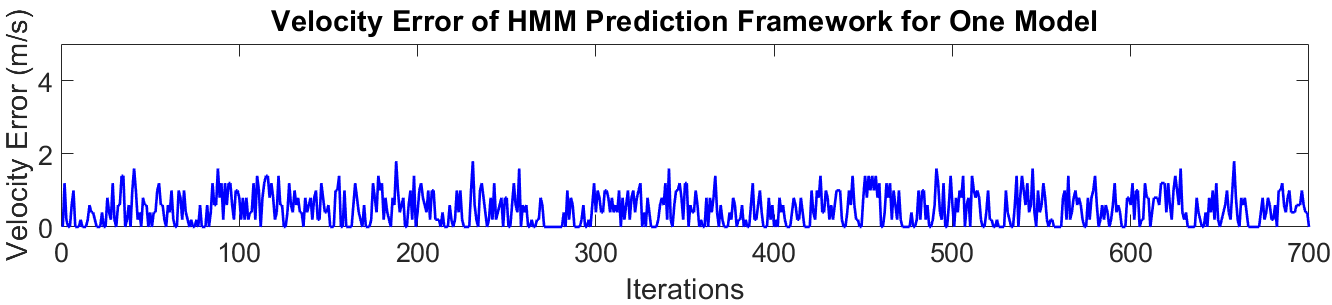
\includegraphics[width=\linewidth]{fig/trainvelerror.png}}
	\subfigure[The error between the position of the actual model and estimated positions \label{fig:trainpos}]{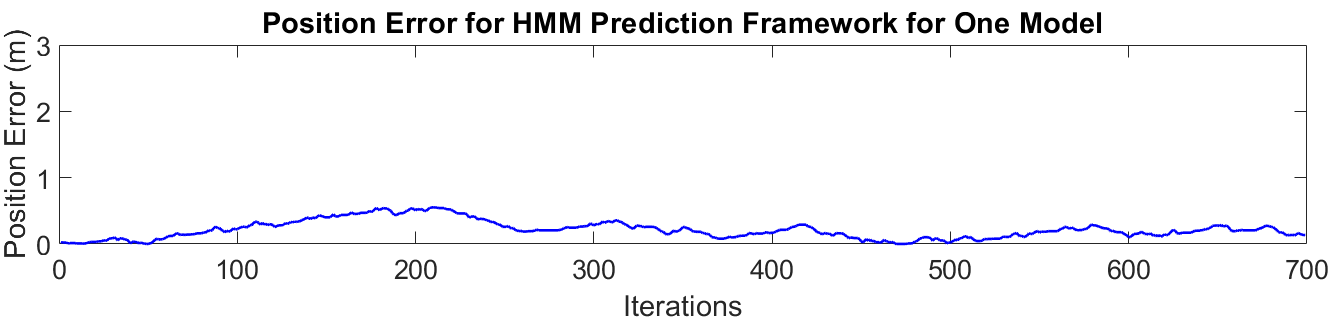
\includegraphics[width=\linewidth]{fig/trainposerror.png}}
	\vspace{-10pt}
	\caption{Error of Model Training}
	\label{fig:trainerrors}
	\vspace{-10pt}
\end{figure}


Fig.~\ref{fig:train2} shows the training and online prediction (starting at 700 iterations) relative to lane changes. During the prediction phase the RMSE was recorded as $1.2564$m. These errors are due to the fact that the trained vehicles and measurements were noisy to consider a more realistic behavior. These results validate that the proposed framework is able to predict efficiently future velocity and lane change states, given a pre-trained model.

\begin{figure}[ht]
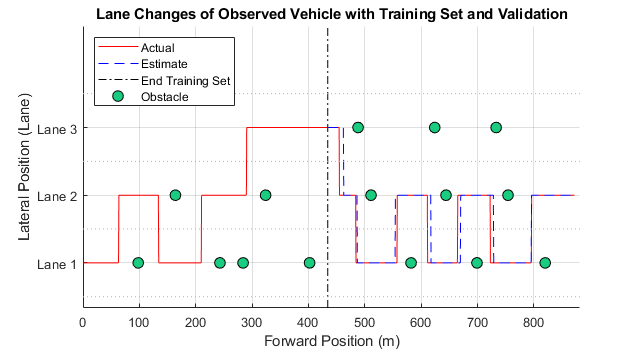
\includegraphics[width=0.48\textwidth]{fig/train2.png}
 \vspace{-10pt}
\caption{Lane change training and prediction. Online prediction is occurring at 700 iterations} \label{fig:train2}
\end{figure}
	\vspace{-10pt}
\subsection{Model Fitting Example}

Building on the previous results, here we demonstrate the model fitting approach presented in Section \ref{sec:omf}. For the sake of simplicity in this work, we trained and built 3 different vehicles models whose velocities were between $22$m/s and $32$m/s. Specifically, one vehicle was aggressive, one was conservative, and the third vehicle's behavior was in between the other two behaviors. Three different transition and emission matrices were computed offline and used online to predict the behavior of a new vehicle with the assumption that this new vehicle's model was similar to one of the previously sampled behaviors. Following the procedure in Section \ref{sec:omf} at each iteration, a model for the new vehicle is built and compared with each of the pre-trained models. The model with the minimum error (i.e. with the highest trust) is selected at each iteration to predict future states of the new vehicle.

Fig.~\ref{fig:error} shows the error between the model of the vehicle and each pre-trained model, Fig.~\ref{fig:trust} shows the trust at each iteration, while Fig.~\ref{fig:select} displays the choice of model at every iteration. As expected, the error is high at the beginning because fewer transitions are observed which are very likely to be similar among different models. As the simulation advances and more data are gathered, trust increases and the error decreases aligning the prediction with one of the three pre-trained models, which, in this case, was Model 2. Convergence is achieved in about 300 iterations.  

\begin{figure}[ht!]
	\centering
	\subfigure[Fit error between the current vehicle and each of the three pretrained models \label{fig:error}]{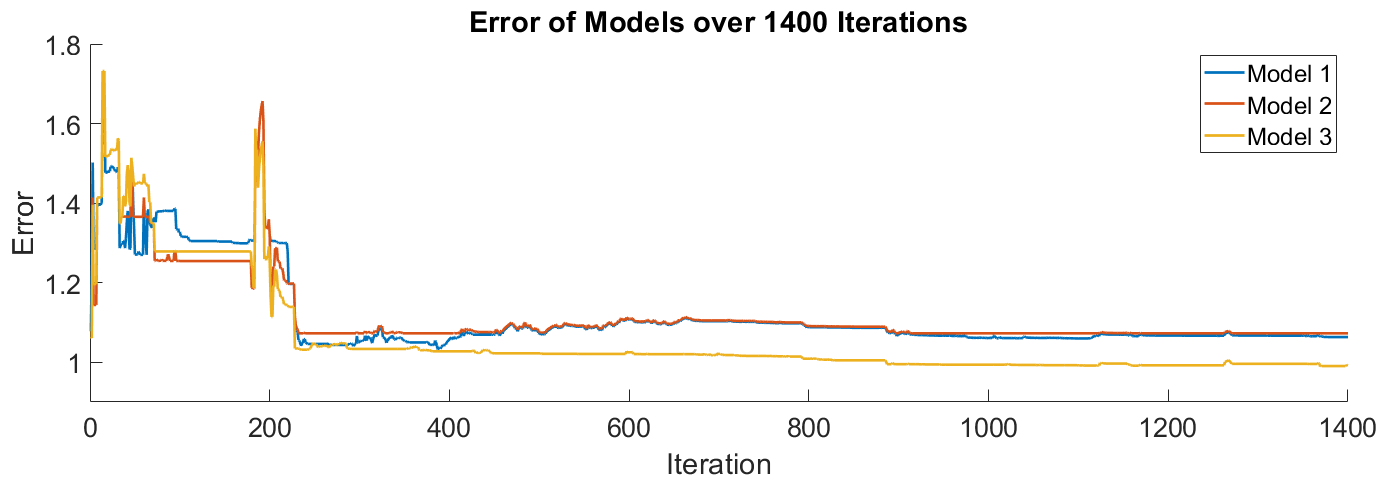
\includegraphics[width=\linewidth]{fig/modelerror.png}}
	\subfigure[Trust associated with the best-fit model at each iteration
	\label{fig:trust}]{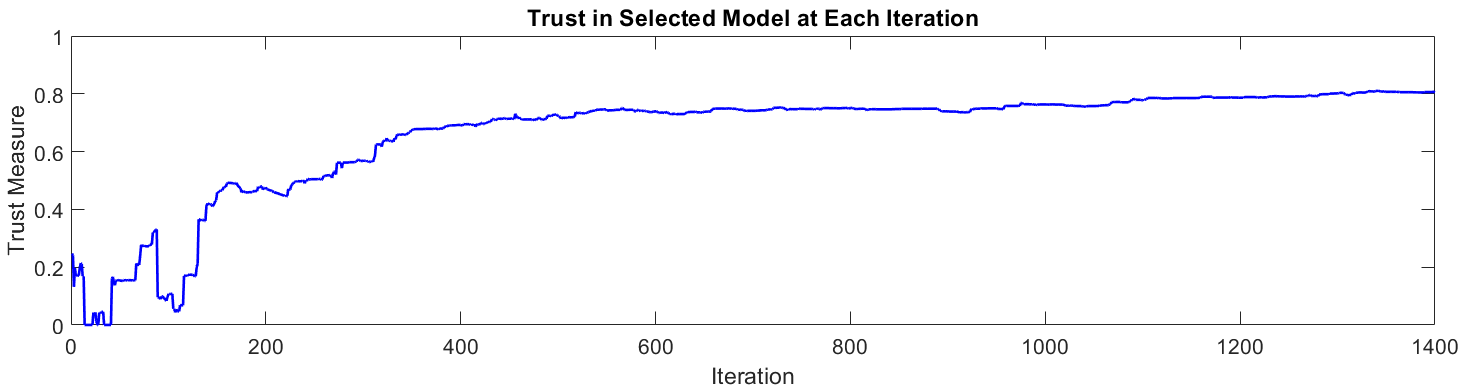
\includegraphics[width=\linewidth]{fig/trustfit.png}}
	\subfigure[The selected model at each iteration
	\label{fig:select}]{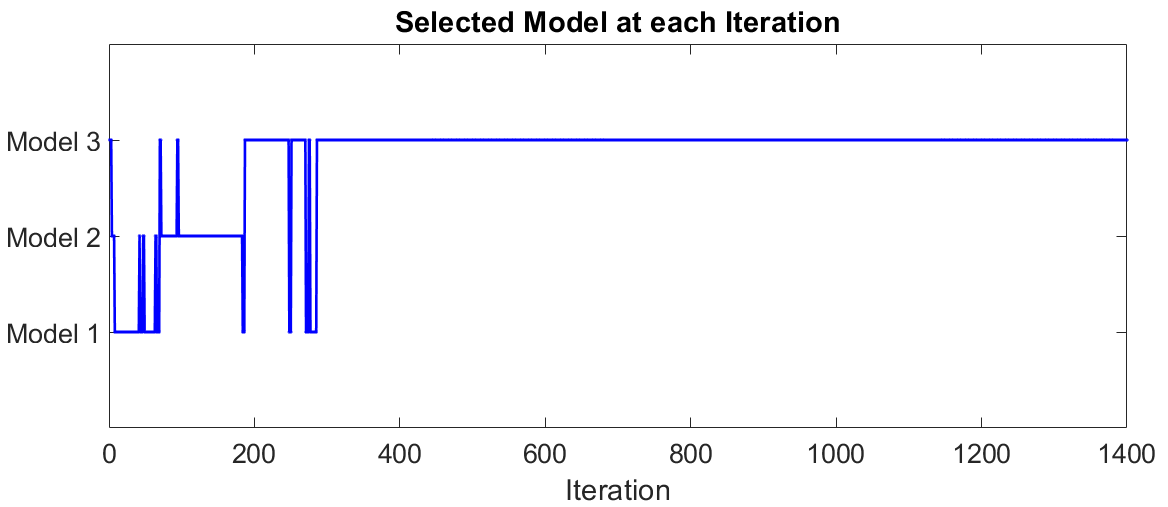
\includegraphics[width=\linewidth]{fig/modelselect.png}}
	\vspace{-0pt}
	\caption{Model Selection Process: Model Error, Trust Measure, and Selection}
	\label{fig:fitprocess}
	\vspace{-0pt}
\end{figure}

Fig.~\ref{fig:fwd} shows the error between the predicted and actual velocity of the vehicle. The RMSE of this trial was recorded as $1.1423$m/s.
Fig.~\ref{fig:lanchan} shows the lane change behavior. The RMSE between the prediction and the actual lane change actions was recorded as $3.521$m.

Using the selected model, we are able to make predictions for every iteration of run-time. In Fig.~\ref{fig:fwd}, we show the accuracy of the fit for velocity/forward position over 1400 iterations. The RMSE of this trial was $2.1423$m/s. 
In Fig.~\ref{fig:lanchan}, we show the predictions made that pertain to lane changes and following distance. The RMSE of the predictions as compared to the actual actions was $3.521$m. 

\begin{figure}[ht!]
    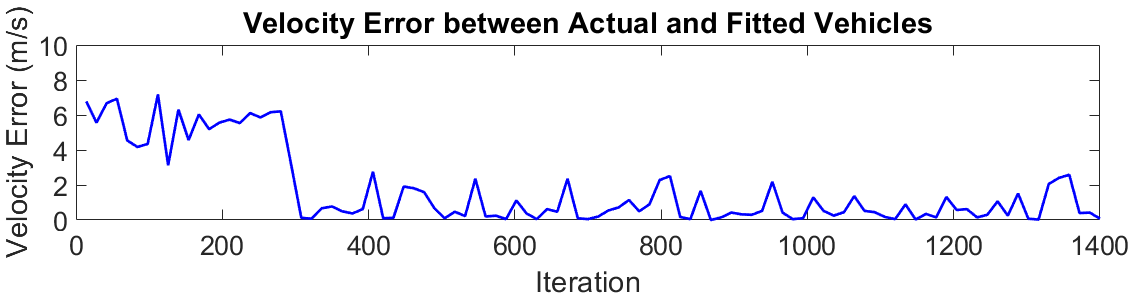
\includegraphics[width=0.48\textwidth]{fig/fiterroravg.png}
    \vspace{-0pt}
    \caption{Absolute Error of velocity between the fitted and actual vehicles} \label{fig:fwd}
\end{figure}
% \vspace{-5pt}
\begin{figure}[ht!]
    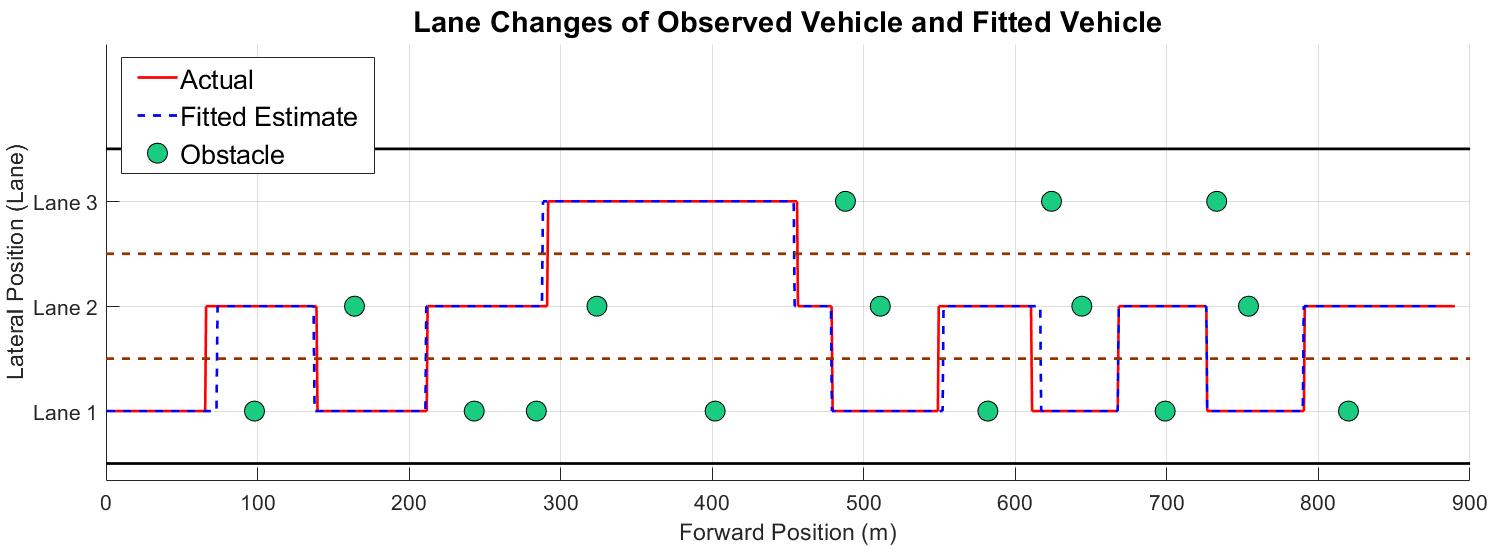
\includegraphics[width=0.48\textwidth]{fig/lanefit.png}
     \vspace{-0pt}
    \caption{The lane changes of the actual vehicle and the best-fit vehicle model} \label{fig:lanchan}
    	     \vspace{-0pt}
\end{figure}
%     \vspace{-5pt}


\subsection{Assistive Planning and Control Case Study}
In order to show the impact of our assistive control, we simulate a scenario similar to the one depicted in Fig.~\ref{fig:hiway}. 
Fig.~\ref{fig:critpt} shows the setup used for this simulation. Two vehicles $q_1$ and $q_2$ with different behaviors are fitted online with the correct model and a HAV $h$ is monitoring and predicting their behavior assessing risk over a 3 time steps horizon. 
Fig.~\ref{fig:critrd} shows the resulting risk over the reachable set of $h$. A user set $r_{\max} = 0.85$ is considered here. As can be noted the risk is increasing at $t+3$ on lane 2 because in this specific case $h$ gets closer to $q_2$ as time advances. 
%We show one case where the user has full control of the HAV, and one where assistance is given to the user. Depicted in Fig.~\ref{fig:critpt} is a scenario where the risk, $r_h\in\hat{\mathcal{R}}$ is nearing the user set limit of $r_{\max} = 0.85$.


\begin{figure}[ht!]
	\centering
	\subfigure[Risk Distribution
	\label{fig:critrd}]{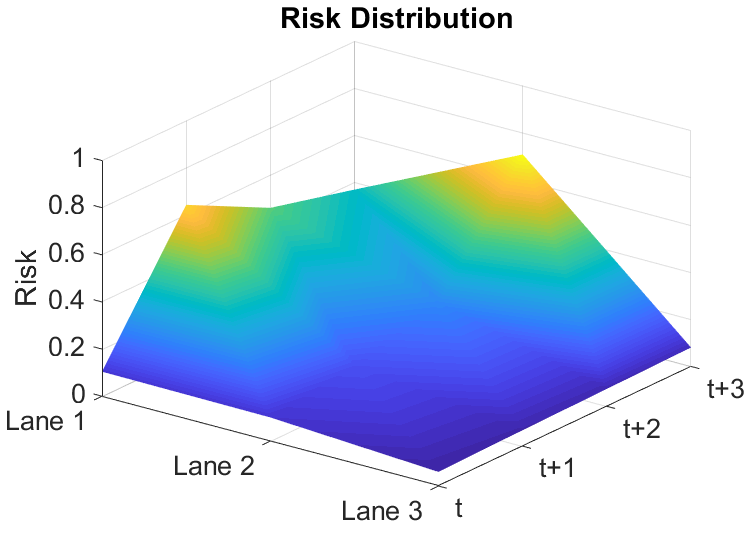
\includegraphics[width=.49\linewidth]{fig/critpt_rd.png}}
	\subfigure[Road Scenario
	\label{fig:critrs}]{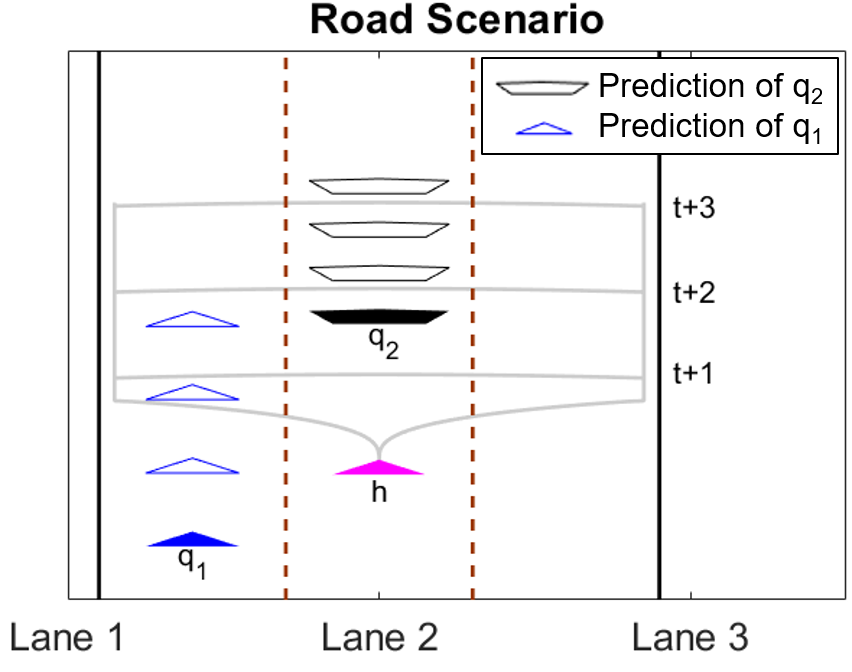
\includegraphics[width=.43\linewidth]{fig/critpt_rs.png}}
	\vspace{-0pt}
	\caption{Example scenario in which $h$ (magenta colored) is monitoring and predicting the behavior of two vehicles $\{q_1,q_2\}$ (blue and black colored).}
	\label{fig:critpt}
	\vspace{-0pt}
\end{figure}

%In Fig.~\ref{fig:critpt}, the magenta vehicle in the center is the HAV we are able to control. The reachable set is shown coming out of the HAV, with the lines marked with $(t+1,t+2,t+3)$. In this case, we are only showing the reachable set and risk distribution for $v_h$. The situation depicted is one of a critical point, which means that a decision has to be made at this time, or there's a heightened chance a collision will occur within $H$. 


In Fig.~\ref{fig:noassist}, we show a snapshot for a situation in which the user was not assisted, i.e., $u^*=u_h, \;\;\forall t>0$. In this scenario, the user reaches the a safety-critical point as in Fig.~\ref{fig:critpt}, and decides to avoid $q_2$, by moving to the left lane $l_1$, where the risk is high (as shown in Fig.~\ref{fig:critrd}). As a result a collision happened in this case.

\begin{figure}[ht!]
	\centering
	\subfigure[Risk Distribution
	\label{fig:noasstrd}]{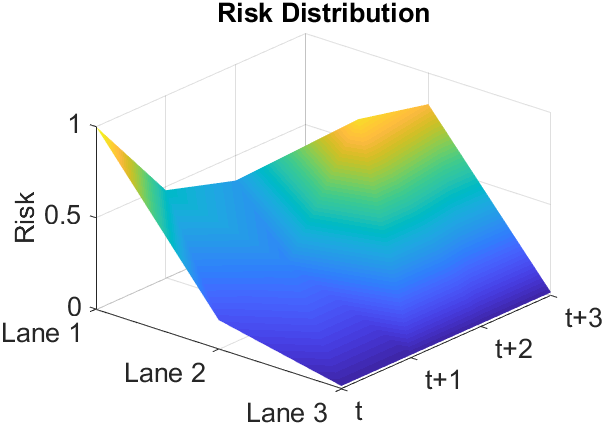
\includegraphics[width=.49\linewidth]{fig/noassist_rd.png}}
	\subfigure[Road Scenario
	\label{fig:noasstrs}]{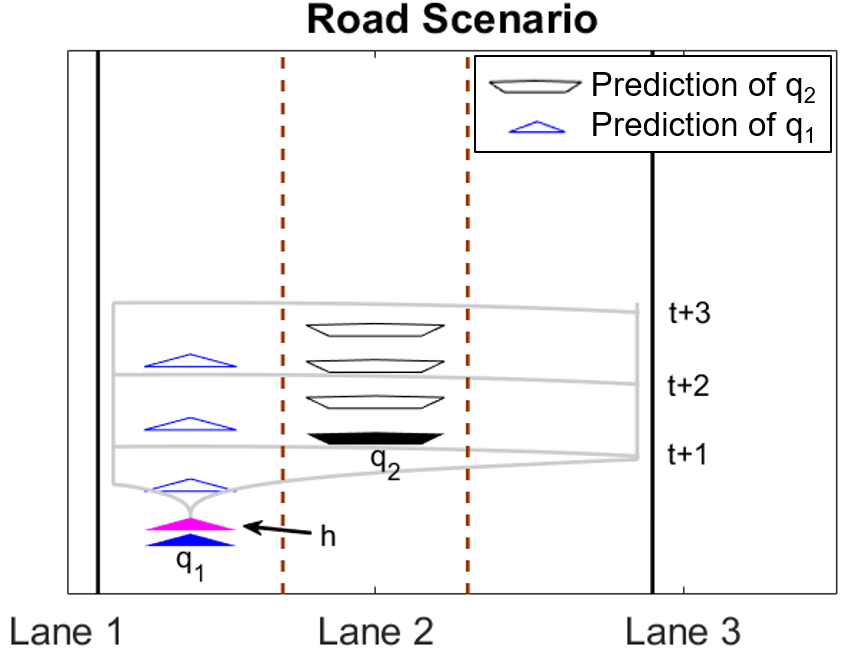
\includegraphics[width=.43\linewidth]{fig/noassist_rs.png}}
	\vspace{-0pt}
	\caption{Unassisted - Risk Distribution and Road Scenario}
	\label{fig:noassist}
	\vspace{-0pt}
\end{figure}
In our approach, we aim to avoid such a situation. Fig.~\ref{fig:assistrs} shows a snapshot of the same scenario but this time with the assistive behavior enabled. In this case the optimal input was switched between $u_h$ and $u_a$ when the risk was above $r_{max}$. 
The user input was modeled the same as in Fig.~\ref{fig:noassist}, but in this case, the assistive input was taken into account as the risk surpassed $r_{\max}$. Using our framework, the $u_h$ was overwritten by $u_a$ guaranteeing a safe operation of $h$.

\begin{figure}[ht!]
	\centering
	\subfigure[Risk Distribution
	\label{fig:assistrd}]{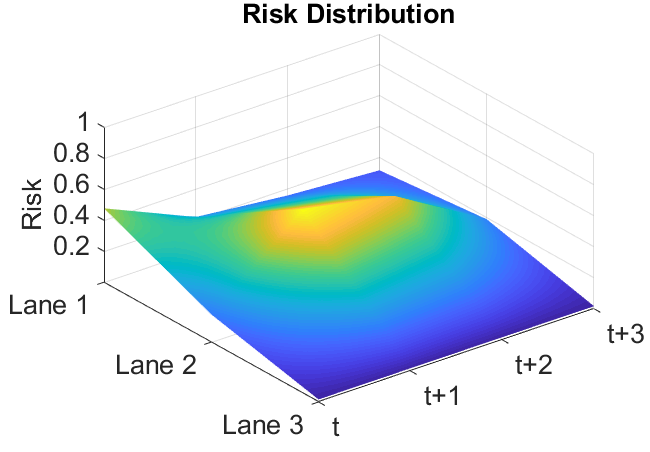
\includegraphics[width=.49\linewidth]{fig/assist_rd.png}}
	\subfigure[Road Scenario
	\label{fig:assistrs}]{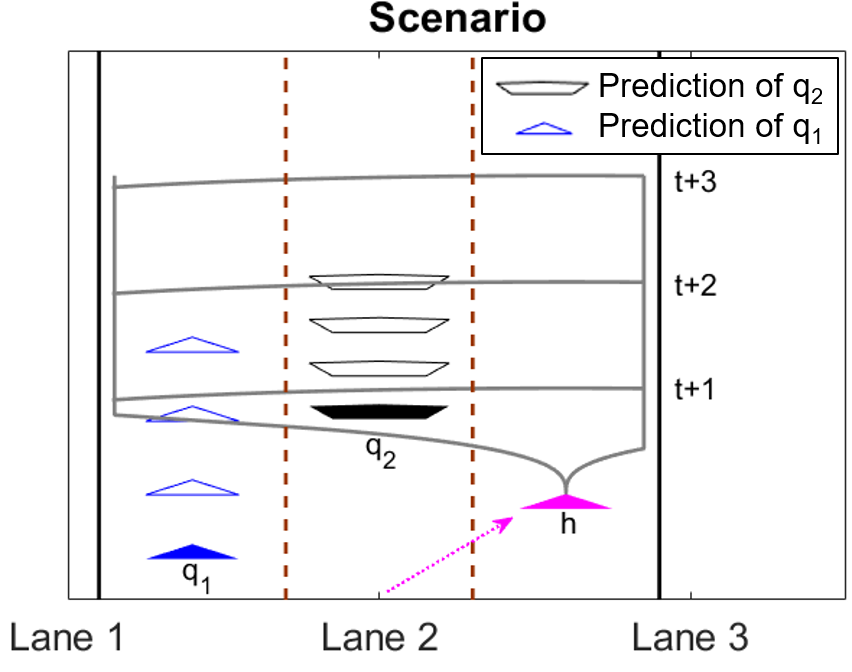
\includegraphics[width=.43\linewidth]{fig/assist_rs.png}}
	\vspace{-0pt}
	\caption{Assisted - Risk Distribution and Road Scenario}
	\label{fig:assist}
	\vspace{-0pt}
\end{figure}


Animations for the simulations presented above can be found at https://www.bezzorobotics.com/rp-acc19.

\section{Conclusions} \label{sec:concs}
%\NB{conclusions should summarize what we have accomplished with this work and what you learned from this work, including the pros and cons. They need to discuss also current and future directions.}
In this work, we have presented an approach for simultaneously predicting the future states of multiple vehicles and assisting the user of an HAV. Our approach uses a Hidden Markov Model-based framework to build offline models of different vehicles and to fit these models to any number of online observed vehicles. A shared control scheme was also presented to ensure that the user of an HAV does not enter an unsafe state. We were able to show that by minimizing our predicted risk at each step, we are able to ensure the vehicle stays as safe as possible. While the prediction method is reliable, model fitting is most effective when the set of offline models is rich and varied enough such that any vehicle can be fitted accurately.

In future work, we will build more pre-trained models to increase richness. In this paper, we are primarily concerned with the technique. In the future, we plan to further expand the prediction framework to different situations, which would involve more realistic dynamics and other factors, such as external disturbances. In addition, we plan to expand our framework across different types of vehicles and other cyber-physical systems.

\section{Acknowledgement}

This material is based upon work supported by NSF under grant number \#1816591 and 
the Air Force Research Laboratory and the Defense Advanced Research Projects Agency under Contract No. FA8750-18-C-0090. 

%\NB{KEEP THIS - this sentence needs more explanation. If we don't have enough models we need to mention that future work is centered on using existing models to extract new models}
% references section

% can use a bibliography generated by BibTeX as a .bbl file
% BibTeX documentation can be easily obtained at:
% http://mirror.ctan.org/biblio/bibtex/contrib/doc/
% The IEEEtran BibTeX style support page is at:
% http://www.michaelshell.org/tex/ieeetran/bibtex/
%\bibliographystyle{IEEEtran}
% argument is your BibTeX string definitions and bibliography database(s)
%\bibliography{IEEEabrv,../bib/paper}
%
% <OR> manually copy in the resultant .bbl file
% set second argument of \begin to the number of references
% (used to reserve space for the reference number labels box)

%\begin{thebibliography}{1}

%\bibitem{IEEEhowto:kopka}
%H.~Kopka and P.~W. Daly, \emph{A Guide to \LaTeX}, 3rd~ed.\hskip 1em %plus
%  0.5em minus 0.4em\relax Harlow, England: Addison-Wesley, 1999.
  
  
%\end{thebibliography}

%\printbibliography
%\bibliographystyle{abbrv}
\bibliographystyle{IEEEtran}
\bibliography{mybibliography.bib}


% that's all folks
\end{document}


